\documentclass[aspectratio=169,11pt]{beamer}
% ==========================================================================
%  KSA lecture-slide theme  =  stock beamer "Boadilla"  +  KSA colour theme
%  brand colours sampled from the official KSA symbol mark:
%    Deep Prussian Blue  #2E3192   (지성 - intellect)
%    Golden Gray         #D6CBB1   (감성 - sensibility)
%  Engine: XeLaTeX.  Usage:
%    \documentclass[aspectratio=169,11pt]{beamer}
%    \input{../../theme/ksa-theme.tex}
%  Each deck lives in its own slides/kor/<deck>/ folder together with its
%  own images; ../../figs/ is kept only as a fallback for the shared cache.
% ==========================================================================

\usepackage{fontspec}
\usepackage{amsmath,amssymb}
\usepackage{graphicx}
\graphicspath{{figs/}{./}{../../../figs/}}
\usepackage{booktabs}
\usepackage{listings}
\usepackage{varwidth}

% ---- fonts (no ctex/xeCJK on this box -> fontspec drives CJK directly) -----
\defaultfontfeatures{Ligatures=TeX}
\setmainfont{Noto Sans CJK KR}
\setsansfont{Noto Sans CJK KR}
\setmonofont{Noto Sans Mono CJK KR}[Scale=0.92]

% ---- base theme: stock Boadilla ------------------------------------------
\usetheme{Boadilla}
\usefonttheme{professionalfonts}
\setbeamertemplate{navigation symbols}{}

% ---- KSA colour theme (recolour the stock theme) --------------------------
\definecolor{ksablue}{HTML}{2E3192}
\definecolor{ksabluedk}{HTML}{20226A}
\definecolor{ksagold}{HTML}{D6CBB1}
\definecolor{ksagolddk}{HTML}{A9976B}
\definecolor{ksared}{HTML}{C0392B}
\definecolor{ksagray}{HTML}{5B5B5B}

\setbeamercolor{structure}{fg=ksablue}
\setbeamercolor{alerted text}{fg=ksared}

\setbeamercolor{palette primary}{fg=white,           bg=ksablue}
\setbeamercolor{palette secondary}{fg=white,         bg=ksablue!85!black}
\setbeamercolor{palette tertiary}{fg=white,          bg=ksabluedk}
\setbeamercolor{titlelike}{fg=ksablue}
\setbeamercolor{frametitle}{fg=ksablue,bg=}
\setbeamercolor{title}{fg=ksablue}
\setbeamercolor{author}{fg=ksagray}
\setbeamercolor{institute}{fg=ksagray}
\setbeamercolor{block title}{fg=white,bg=ksablue}
\setbeamercolor{block body}{fg=black!85,bg=ksablue!6}
\setbeamercolor{item}{fg=ksablue}
\setbeamercolor{section in toc}{fg=black!85}

\setbeamerfont{frametitle}{series=\bfseries}
\setbeamerfont{title}{series=\bfseries}

% ---- footline:  KSA mark | "Made by ..." | n / N   (matches reference) ----
\newcommand{\ksacredit}{}
\setbeamertemplate{footline}{%
  \hbox{%
    \begin{beamercolorbox}[wd=.18\paperwidth,ht=2.6ex,dp=1.5ex,leftskip=1.1em]{}%
      \raisebox{-0.35ex}{\includegraphics[height=2.0ex]{ksa-logo.png}}%
    \end{beamercolorbox}%
    \begin{beamercolorbox}[wd=.64\paperwidth,ht=2.6ex,dp=1.5ex,center]{}%
      {\scriptsize\color{ksagray}\ksacredit}%
    \end{beamercolorbox}%
    \begin{beamercolorbox}[wd=.18\paperwidth,ht=2.6ex,dp=1.5ex,rightskip=1.1em]{}%
      \hfill{\scriptsize\color{ksablue}\insertframenumber\,/\,\inserttotalframenumber}%
    \end{beamercolorbox}%
  }%
  \vskip2pt
}

% ---- section divider: stock \sectionpage, KSA-coloured -------------------
\setbeamertemplate{section page}{%
  \begingroup\centering
    {\color{ksagolddk}\rule{0.16\paperwidth}{1pt}}\par\vskip1.0em
    {\usebeamerfont{title}\color{ksablue}\insertsectionhead\par}\vskip1.0em
    {\color{ksagolddk}\rule{0.16\paperwidth}{1pt}}\par
  \endgroup
}
\AtBeginSection[]{\begin{frame}[plain,noframenumbering]\vfill\sectionpage\vfill\end{frame}}

% ---- code listings ------------------------------------------------------------
\lstdefinestyle{ksa}{%
  basicstyle=\ttfamily\scriptsize,
  keywordstyle=\color{ksablue}\bfseries,
  commentstyle=\color{ksagray}\itshape,
  stringstyle=\color{ksagolddk},
  numberstyle=\tiny\color{ksagray},
  backgroundcolor=\color{ksablue!6},
  frame=leftline, framerule=1.4pt, rulecolor=\color{ksablue},
  xleftmargin=1em, aboveskip=0.8em, belowskip=0.4em,
  showstringspaces=false, breaklines=true, language=Python,
}
\lstset{style=ksa}

% ---- handy macros -----------------------------------------------------------
\newcommand{\kb}[1]{\textbf{\color{ksablue}#1}}   % blue keyword
\newcommand{\kq}[1]{\textbf{\color{ksared}#1}}    % red key-question

\setbeamerfont{title}{series=\bfseries,size=\fontsize{24}{30}\selectfont}
\setbeamerfont{subtitle}{series=\bfseries,size=\fontsize{14}{18}\selectfont}
\setbeamerfont{author}{size=\normalsize}
\setbeamerfont{institute}{size=\small}
\graphicspath{{figs/}{../../../../assets/}}
\makeatletter
\newcommand{\markpage}[1]{\protected@write\@auxout{}{\string\newlabel{#1}{{\the\c@framenumber}{}}}\hypertarget{#1}{}}
\newcommand{\pref}[1]{\hyperlink{#1}{\textcolor{ksagolddk}{(p.\ref{#1})}}}
\makeatother

\renewcommand{\ksacredit}{Machine Learning 1 \,\textperiodcentered\, 교차 엔트로피}
\title{교차 엔트로피 (Cross-Entropy)}
\subtitle{확신하고 틀리면 크게 벌 받는다}
\author{Machine Learning 1}
\institute{한국과학영재학교 (KSA)}
\date{}
\begin{document}
\begin{frame}[plain,noframenumbering]\titlepage\end{frame}

% --- 오늘의 질문
\begin{frame}{오늘의 질문}
\vfill
\centering
\includegraphics[width=0.84\linewidth]{ce_hook.png}\par\vskip0.6em
{\large 고양이 사진을 보고 ``강아지 99\%''라고 확신한 AI. 벌점을 몇 점 줘야 할까?}
\vfill
\note{고양이 사진을 보여 줬더니 AI가 강아지일 확률 99퍼센트라고 확신했습니다. 틀렸죠. 그러면 벌점을 몇 점 줘야 할까요? 그냥 틀렸으니 1점? 아니면 확신하고 틀렸으니 더 크게? 분류 모델을 학습시키려면 이 벌점, 즉 손실 함수를 정해야 합니다. 오늘은 분류에서 거의 표준으로 쓰는 벌점, 교차 엔트로피를 배웁니다.}
\end{frame}

% --- 칩 게임
\begin{frame}{칩 100개를 나눠 걸기}
\vfill
\centering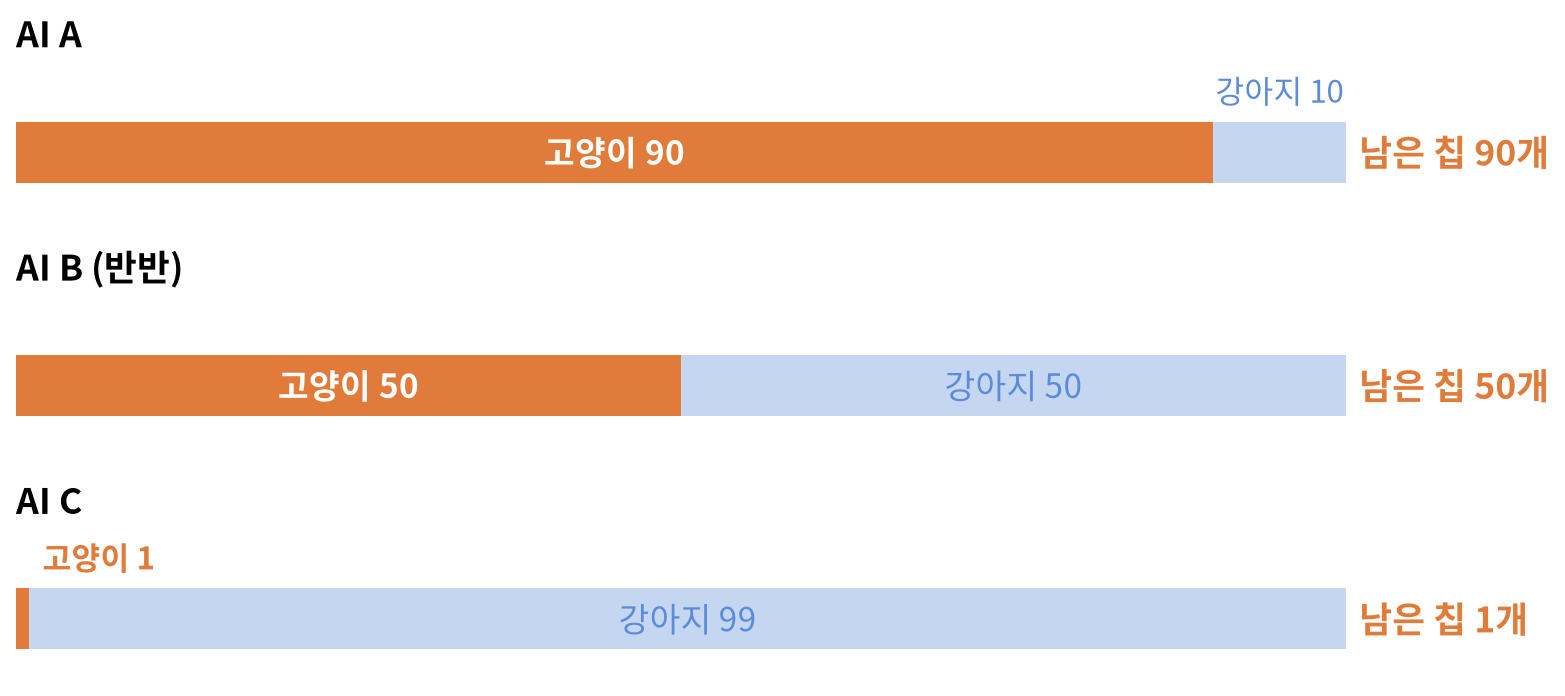
\includegraphics[width=0.8\linewidth]{ce_chips.png}\par\vskip0.4em
{\large AI는 칩 100개를 답마다 나눠 건다. \kq{정답 쪽에 건 칩만 남는다}}
\vfill
\note{AI의 예측을 게임으로 바꿔 봅시다. AI는 칩 100개를 고양이와 강아지에 나눠 겁니다. 고양이 90퍼센트라는 예측은 고양이에 90개, 강아지에 10개를 건 것입니다. 정답이 공개되면 정답 쪽에 건 칩만 남습니다. 정답이 고양이니까 A는 90개, 반반 건 B는 50개, 강아지 99퍼센트라고 한 C는 1개만 남습니다. 남은 칩이 적을수록 큰 벌점을 주면 됩니다.}
\end{frame}

% --- 벌점 곡선
\begin{frame}{남은 칩이 적을수록 큰 벌점}
\markpage{curve}
\vfill
\begin{columns}[c]
\begin{column}{0.58\textwidth}\centering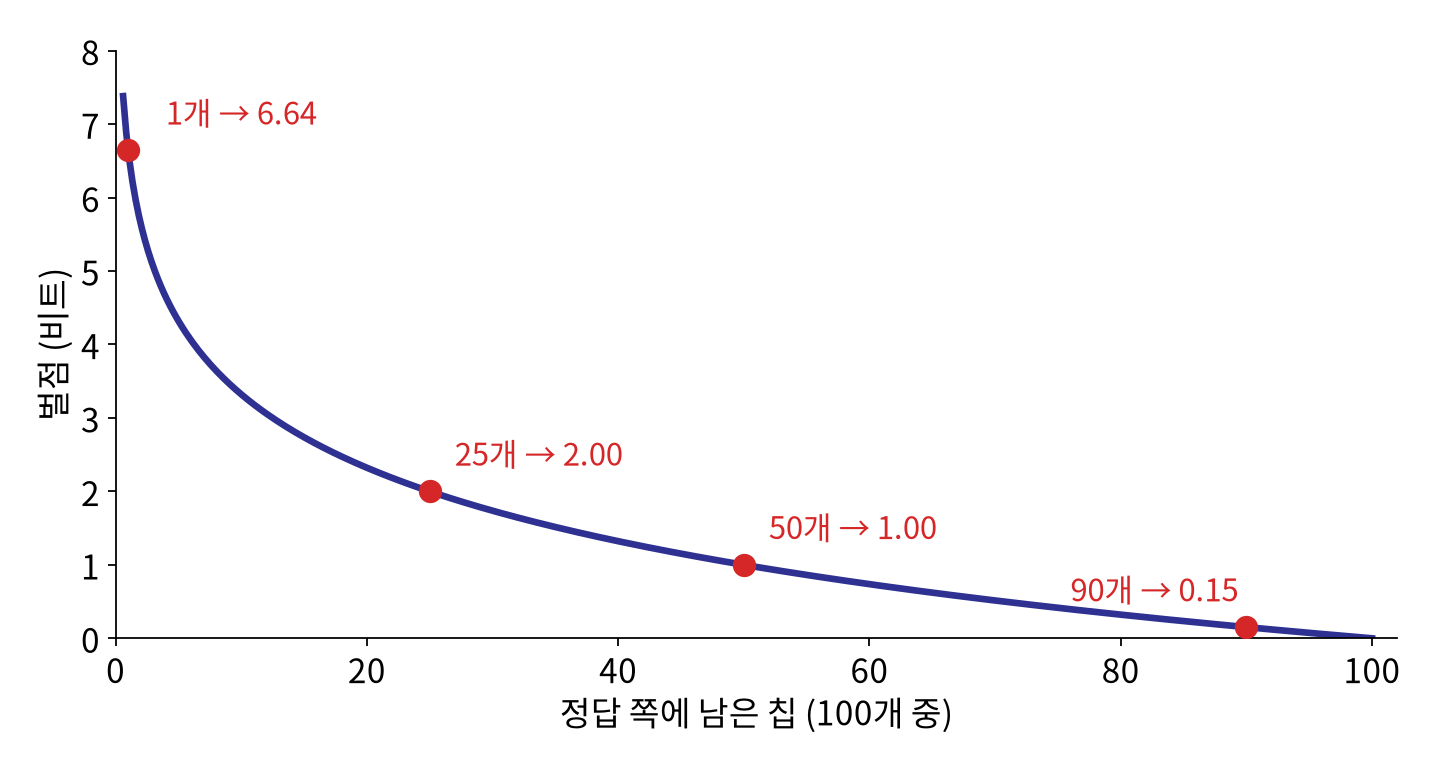
\includegraphics[width=\linewidth]{ce_curve.png}\end{column}
\begin{column}{0.38\textwidth}
{\Large\[ \text{벌점} = -\log_2 \frac{\text{남은 칩}}{100} \]}\vskip0.6em
100개 $\to$ 0 \quad 50개 $\to$ 1 \quad 25개 $\to$ 2\\[0.3em]
\kb{칩이 절반이 될 때마다 벌점 +1}\\[0.8em]
90개 $\to$ \textbf{0.15} \qquad 1개 $\to$ \kq{6.64}\\[0.8em]
{\small 밑은 아무거나: $\log_2$ $\to$ \textbf{비트}, \; $\ln$ $\to$ \textbf{냇}\\ ML 코드는 보통 $\ln$. 값만 상수배 (6쪽)}
\end{column}
\end{columns}
\vfill
\note{벌점은 남은 칩 비율에 마이너스 로그 2를 씌운 값입니다. 다 남으면 0점, 절반이 남으면 1점, 4분의 1이 남으면 2점입니다. 칩이 절반으로 줄 때마다 벌점이 1씩 오릅니다. 그래서 90개 남은 A는 0.15점, 1개 남은 C는 6.64점입니다. 100개에서 1개가 되려면 절반을 6.6번 해야 하니까요. 처음 질문의 답이 6.64점입니다. 한 가지 짚어 두면, 로그의 밑이 꼭 2일 필요는 없습니다. 밑을 바꾸면 값 전체에 같은 상수가 곱해질 뿐이라 어느 AI가 더 나쁜지 순서도, 학습 결과도 같습니다. 밑이 2이면 단위를 비트라고 부르고, 절반마다 1점이라 직관적이어서 오늘 비유에서는 2를 씁니다. 실제 머신러닝 코드는 보통 자연로그를 쓰고, 단위는 냇이라고 합니다.}
\end{frame}

% --- 파산과 반반
\begin{frame}{정답에 0개를 걸었다면}
\vfill
\centering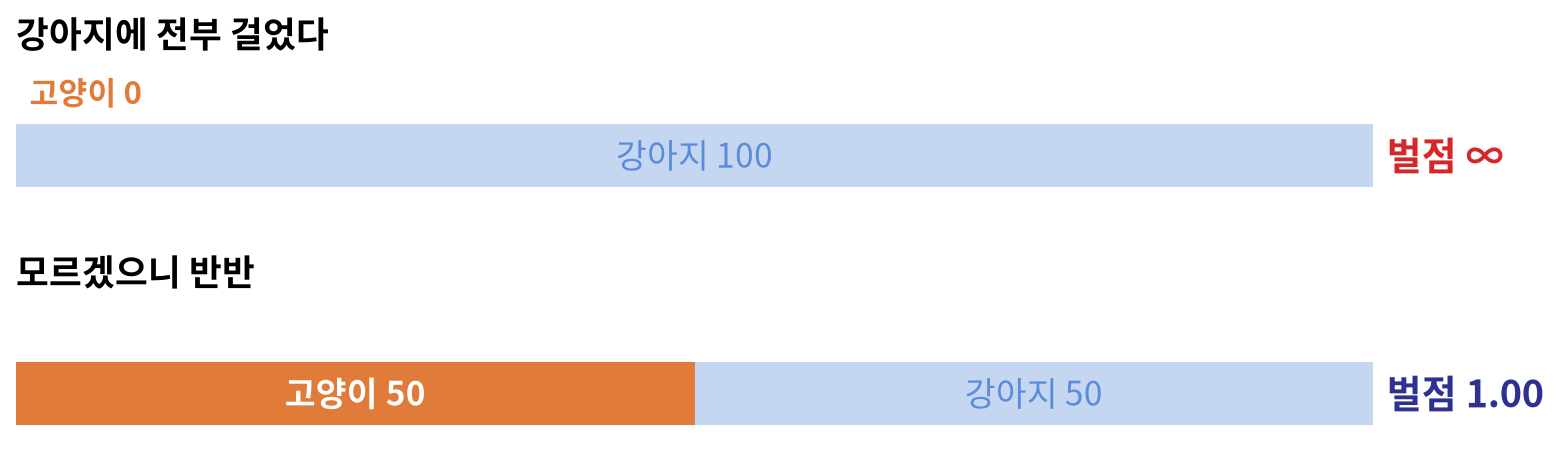
\includegraphics[width=0.8\linewidth]{ce_allin.png}\par\vskip0.6em
{\large 정답에 하나도 안 걸면 \kq{파산: 벌점 $\infty$}. 모를 땐 반반이 낫다 (틀려도 1점)}
\vfill
\note{정답인 고양이에 하나도 안 걸고 강아지에 100개를 다 걸었다면 칩이 하나도 안 남습니다. 파산이고, 로그 0은 마이너스 무한대라서 벌점은 무한대입니다. 그래서 교차 엔트로피로 학습한 모델은 모를 때 함부로 확신하지 않습니다. 반반에 걸면 어느 쪽이 정답이든 1점만 잃기 때문입니다. 확신하고 틀리는 것을 아주 크게 벌하는 벌점입니다.}
\end{frame}

% --- 칩 = 확률
\begin{frame}{칩의 비율 = 확률}
\markpage{formula}
\vfill
\centering
{\Large\[ L = -\log q_{\text{true}} \qquad\Longrightarrow\qquad
H(p, q) = -\sum_{k=1}^{K} \underbrace{p_k}_{\text{true}} \log \underbrace{q_k}_{\text{predicted}} \]}\vskip0.6em
\begin{tabular}{lll}
$q$ & AI가 각 답에 건 칩의 비율 & 예: 고양이 0.01, 강아지 0.99\\[0.2em]
$p$ & 정답 (정답 칸만 1) & 고양이 1, 강아지 0\\[0.2em]
$H(p,q)$ & 교차 엔트로피 & $-(1\cdot\log_2 0.01 + 0\cdot\log_2 0.99) = 6.64$
\end{tabular}\vskip0.6em
{\small 정답 칸만 1이라 합에서 정답 항 하나만 남는다 $\to$ 왼쪽 식}
\vfill
\note{칩의 비율이 곧 확률입니다. AI가 정답에 준 확률을 q라고 하면 벌점은 마이너스 로그 q입니다. 일반적인 식은 오른쪽입니다. p는 정답 분포, q는 AI의 예측 분포이고, 모든 답에 대해 p 곱하기 로그 q를 더해 마이너스를 붙입니다. 분류에서는 정답 칸만 1이고 나머지는 0이라서, 합에서 정답 항 하나만 남고 왼쪽 식이 됩니다. 이 식을 교차 엔트로피라고 부릅니다.}
\end{frame}

% --- 이진 분류
\begin{frame}{로지스틱회귀의 손실이 바로 이것}
\vfill
\centering
{\Large\[ L = -\big[\, y \ln \hat y + (1-y) \ln (1-\hat y) \,\big] \]}\vskip0.4em
$y$: 정답 (1 또는 0) \qquad $\hat y = \sigma(z)$: 1일 확률 (시그모이드 출력)\\[0.8em]
\begin{tabular}{ll}
$y = 1$ 이면 & $L = -\ln \hat y$ \quad (1에 건 칩)\\[0.3em]
$y = 0$ 이면 & $L = -\ln (1-\hat y)$ \quad (0에 건 칩)
\end{tabular}\vskip0.8em
\kb{실제 코드는 $\log_2$ 대신 자연로그 $\ln$} \quad {\small 6.64 비트 $= 6.64 \times \ln 2 \approx 4.60$ (값만 상수배)}
\vfill
\note{2주차 로지스틱회귀에서 쓰는 손실이 바로 이 교차 엔트로피입니다. 답이 두 개뿐이라 y가 1이면 앞 항만, y가 0이면 뒤 항만 남습니다. 결국 정답 쪽에 건 칩에 마이너스 로그를 씌운 것과 같습니다. 한 가지 차이는 로그의 밑입니다. 비유에서는 절반마다 1점이 되도록 로그 2를 썼지만, PyTorch나 scikit-learn은 자연로그를 씁니다. 값이 상수배만 다르고 최솟값의 위치는 같습니다.}
\end{frame}

% --- 왜 MSE 말고
\begin{frame}{왜 오차 제곱(MSE)이 아닐까: 벌점의 크기}
\vfill
\centering
{\large
\begin{tabular}{lcc}
 & \textbf{MSE} $(1-\hat y)^2$ & \textbf{교차 엔트로피} $-\ln \hat y$\\[0.3em]\hline\\[-0.6em]
정답에 0.9 & 0.01 & 0.11\\[0.3em]
반반 0.5 & 0.25 & 0.69\\[0.3em]
\kq{확신하고 틀림 0.01} & \kq{0.98} & \kq{4.60}\\[0.3em]
정답에 0 & 1 (최대) & $\infty$
\end{tabular}}\vskip1.0em
\kq{MSE는 아무리 크게 틀려도 벌점이 1을 넘지 못한다}
\vfill
\note{회귀에서 쓰던 오차 제곱을 분류에도 쓰면 안 될까요? 정답이 1이고 확률 예측을 와이햇라 하면 MSE는 1 빼기 와이햇의 제곱입니다. 확률은 0과 1 사이라서 아무리 크게 틀려도 벌점이 1을 넘지 못합니다. 강아지 99퍼센트라고 확신하고 틀린 AI도 0.98점밖에 안 받습니다. 교차 엔트로피는 4.6점, 정답에 0을 줬다면 무한대입니다. 확신하고 틀린 것을 MSE는 충분히 벌하지 못합니다.}
\end{frame}

% --- 기울기 유도
\begin{frame}{더 큰 이유: 기울기}
\markpage{grad}
\vfill
{\small 정답 $y=1$, \; $\hat y = \sigma(z)$, \; $\dfrac{\partial \hat y}{\partial z} = \hat y(1-\hat y)$ \; (시그모이드의 미분)}\vskip0.6em
\centering
{\large
\begin{align*}
\text{교차 엔트로피:}\quad \frac{\partial L}{\partial z} &= -\frac{1}{\hat y}\cdot \hat y(1-\hat y) = \boldsymbol{\textcolor{ksablue}{-(1-\hat y)}} && \text{약분}\\[0.4em]
\text{MSE:}\quad \frac{\partial L}{\partial z} &= -2(1-\hat y)\cdot \hat y(1-\hat y) && \text{그대로}
\end{align*}}\vskip0.4em
\kq{확신하고 틀려서 $\hat y \approx 0$ 이면, MSE의 기울기는 $\hat y$ 가 곱해져 0에 가깝다}
\vfill
\note{더 큰 이유는 기울기입니다. 출력 와이햇는 z에 시그모이드를 씌운 값이고, 시그모이드의 미분은 와이햇 곱하기 1 빼기 와이햇입니다. 교차 엔트로피는 로그를 미분한 1/와이햇가 시그모이드 미분의 와이햇와 약분되어서, 기울기가 깔끔하게 마이너스 1 빼기 와이햇가 됩니다. 크게 틀릴수록 기울기도 큽니다. MSE는 약분이 안 되고 와이햇가 곱해진 채로 남습니다. 그래서 확신하고 틀려서 와이햇가 0에 가까우면 기울기도 0에 가까워지고, 가장 많이 고쳐야 할 때 학습이 거의 멈춥니다.}
\end{frame}

% --- 기울기 그림
\begin{frame}{그림으로: 손실과 기울기}
\vfill
\centering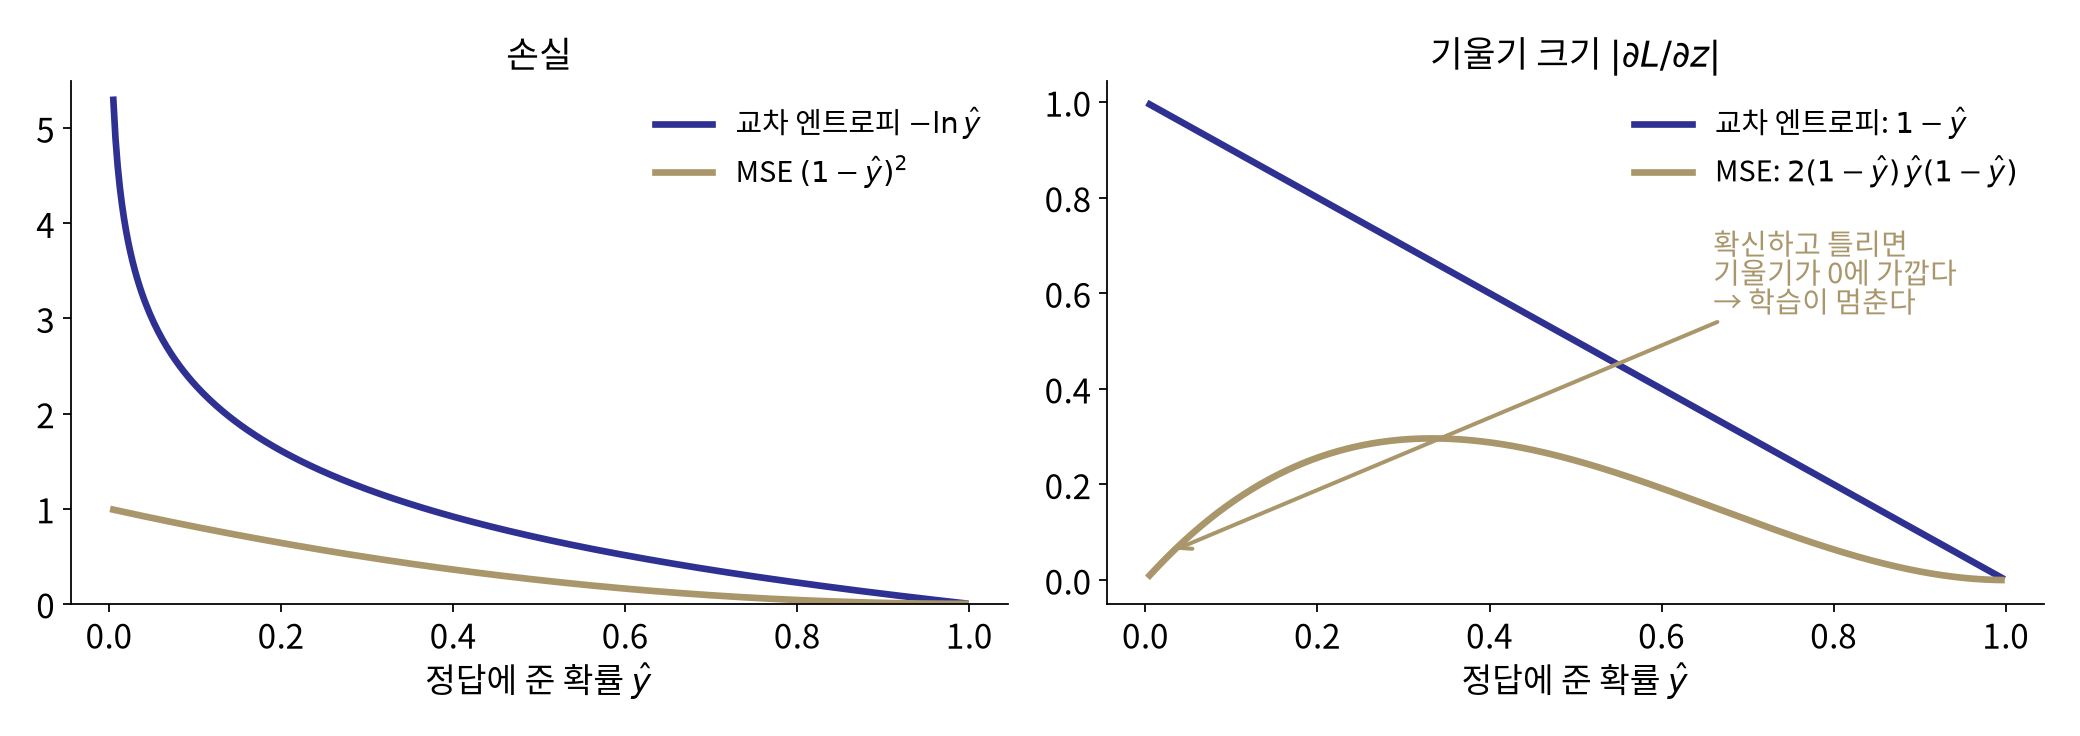
\includegraphics[width=0.92\linewidth]{ce_vs_mse.png}\par\vskip0.3em
{\small 오른쪽: 교차 엔트로피는 틀릴수록 기울기가 크고, MSE는 확신하고 틀린 왼쪽 끝에서 기울기가 사라진다 \pref{grad}}
\vfill
\note{그림으로 보면 차이가 분명합니다. 왼쪽 손실을 보면 교차 엔트로피는 정답 확률이 0에 가까워질수록 끝없이 커지고, MSE는 1에서 멈춥니다. 오른쪽 기울기를 보면 교차 엔트로피는 틀릴수록 기울기가 커지는 직선입니다. MSE는 가운데서 잠깐 커졌다가, 가장 크게 틀린 왼쪽 끝에서 0으로 떨어집니다. 실습에서 이 차이를 실제 데이터로 확인합니다.}
\end{frame}

% --- 학습
\begin{frame}{학습 = 정답 쪽에 칩을 더 거는 과정}
\vfill
\centering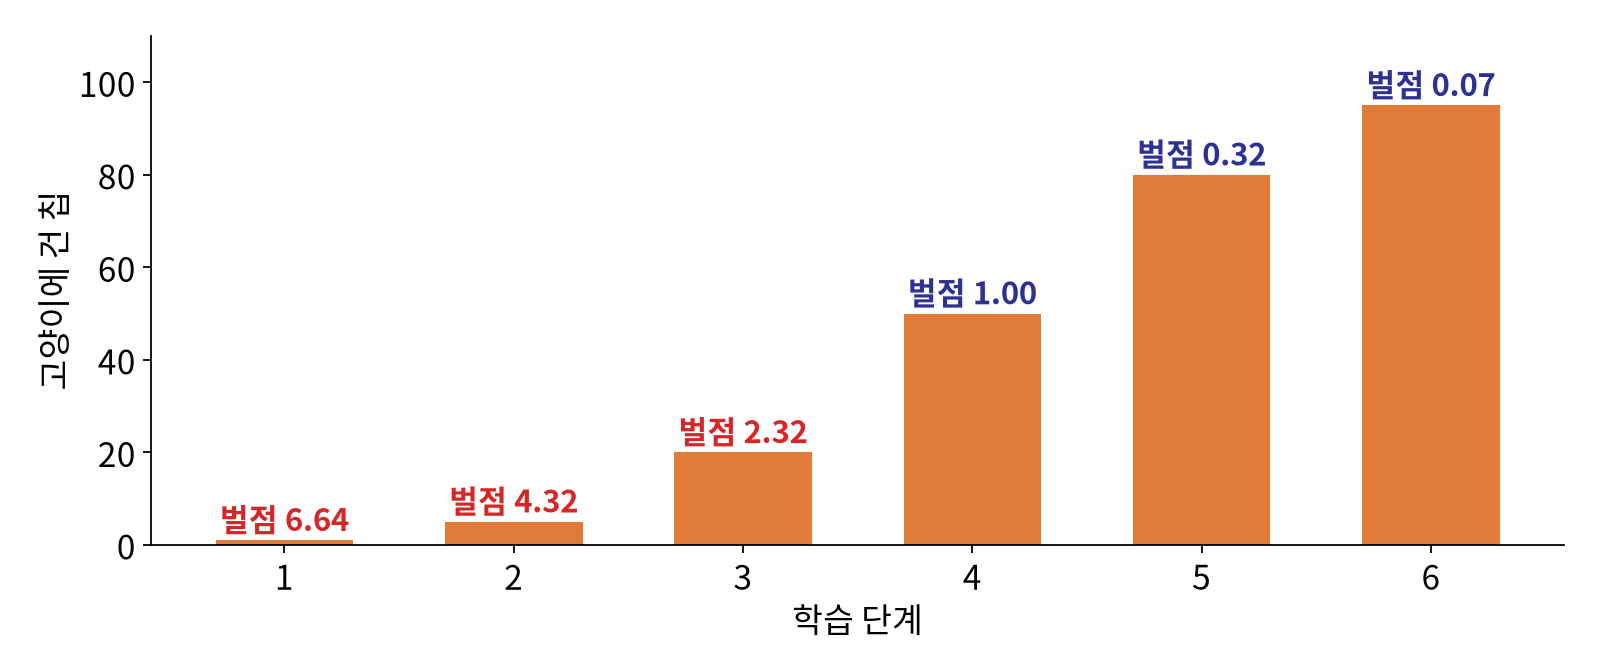
\includegraphics[width=0.78\linewidth]{ce_learning.png}\par\vskip0.3em
{\large 고양이 칩 1개 $\to$ 95개 \quad 벌점 \kq{6.64} $\to$ \kb{0.07}}
\vfill
\note{학습은 경사하강법으로 이 벌점을 줄이는 과정입니다. 칩 비유로 말하면, 정답 쪽에 칩을 점점 더 거는 과정입니다. 처음에는 고양이에 1개만 걸어서 벌점이 6.64였지만, 학습이 진행되면서 5개, 20개, 50개로 늘고 마지막에는 95개, 벌점 0.07까지 내려갑니다. 수많은 사진에 대해 이 벌점의 평균을 줄이는 것이 분류 모델의 학습입니다.}
\end{frame}

% --- 다음 단어
\begin{frame}{챗GPT도 같은 벌점을 받는다}
\vfill
\centering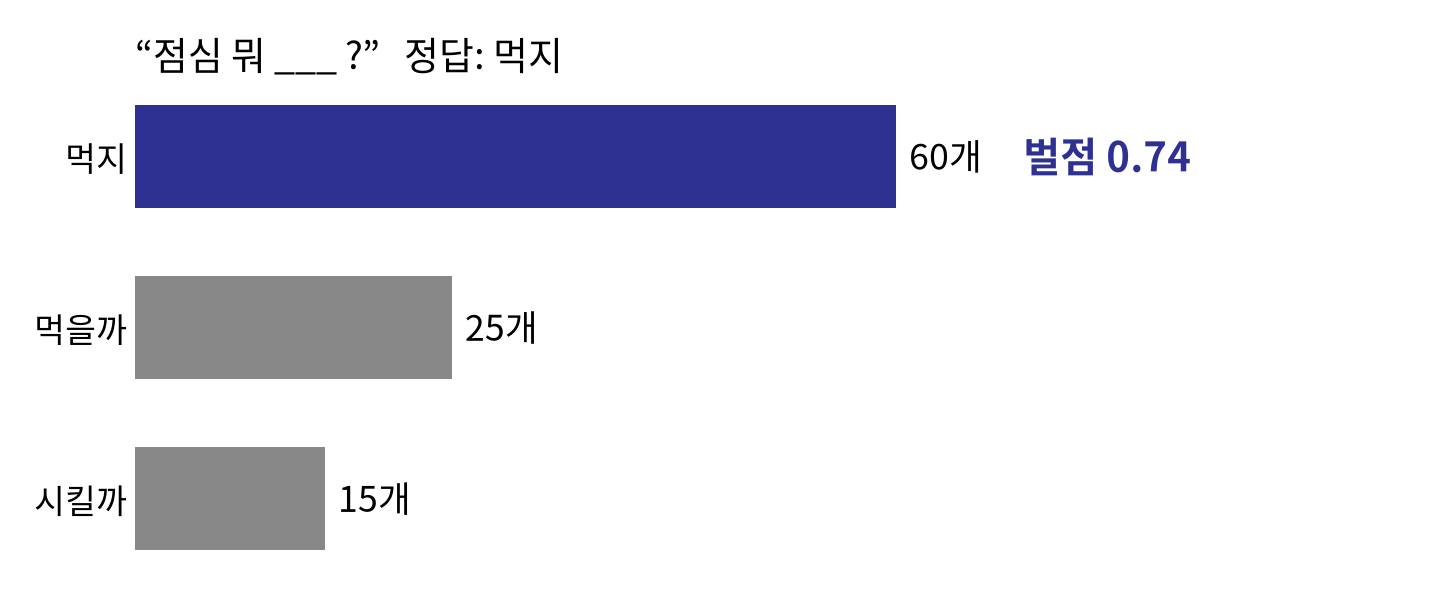
\includegraphics[width=0.7\linewidth]{ce_words.png}\par\vskip0.4em
{\large 다음 단어 후보들에 칩을 나눠 걸고, 정답 단어에 건 칩으로 벌점을 받는다}\\[0.4em]
{\small 언어 모델의 사전학습 = 다음 단어(토큰)의 교차 엔트로피를 줄이는 것 (17주차)}
\vfill
\note{이 벌점은 챗GPT 같은 언어 모델에서도 그대로 쓰입니다. 점심 뭐 다음에 올 단어로 먹지에 60개, 먹을까에 25개, 시킬까에 15개를 걸었다고 합시다. 실제 다음 단어가 먹지라면 60개가 남고 벌점은 0.74입니다. 언어 모델은 인터넷의 엄청난 양의 글에서 다음 단어를 맞히며 이 벌점의 평균을 줄이는 방식으로 학습합니다. 17주차에 다시 만납니다.}
\end{frame}

% --- 문제풀이
\begin{frame}{문제풀이}
\vfill
\begin{enumerate}
\item 칩 100개 중 정답에 25개를 걸었다. 벌점(비트)은?\vskip0.7em
\item 고양이 · 강아지 · 토끼에 칩을 (70, 20, 10)개 걸었다. 정답이 강아지일 때 벌점(비트)은? \; ($\log_2 5 \approx 2.32$)\vskip0.7em
\item 로지스틱회귀에서 $y = 0$, $\hat y = 0.9$. 교차 엔트로피($\ln$)는? \; ($\ln 10 \approx 2.30$)\vskip0.7em
\item 정답에 100개를 다 걸면 벌점은 0이다. 그러면 항상 한쪽에 다 거는 게 좋을까?
\end{enumerate}
\vfill
\note{문제를 풀어 봅시다. 1번 답. 4분의 1이 남았으니 절반을 두 번, 벌점 2입니다. 2번 답. 정답 강아지에 20개, 비율 0.2이므로 마이너스 로그 2의 0.2, 로그 2의 5와 같아서 약 2.32입니다. 3번 답. y가 0이면 뒤 항만 남아 마이너스 ln 1 빼기 0.9, 마이너스 ln 0.1, ln 10과 같아서 약 2.30입니다. 4번 답. 맞으면 0점이지만 틀리면 파산, 벌점 무한대입니다. 평균 벌점을 줄이려면 실제로 맞을 확률만큼 거는 것이 가장 좋습니다. 그래서 교차 엔트로피로 학습한 모델의 출력은 확률처럼 해석할 수 있습니다.}
\end{frame}

% --- 실습
\begin{frame}{실습}
\vfill
\centering\begin{tabular}{rl}
\large 1 & 칩 비유를 코드로: 벌점 손계산 $\to$ scikit-learn \texttt{log\_loss} 와 맞춰 보기\\[0.5em]
\large 2 & 유방암 진단 데이터: 같은 로지스틱회귀를 교차 엔트로피 vs MSE 로 학습해 비교\\[0.5em]
\large 3 & 셰익스피어 글: 다음 글자에 칩 나눠 걸기 (고르게 vs 세어서) 벌점 비교
\end{tabular}\vskip1em
Breast Cancer Wisconsin (569명, scikit-learn 내장) · Tiny Shakespeare (약 100만 글자)\\[0.4em]\href{https://colab.research.google.com/github/SuminHan/book-ml/blob/main/slides/v2/ml1/week02/cross_entropy/lab/cross_entropy.ipynb}{\textcolor{ksagolddk}{▶ Colab에서 실습 노트북 열기}}
\vfill
\note{실습은 세 부분입니다. 첫째, 오늘 손으로 계산한 벌점을 코드로 구현하고 scikit-learn의 log loss와 같은지 확인합니다. 둘째, 유방암 진단 데이터로 같은 로지스틱회귀를 교차 엔트로피와 MSE로 각각 학습시켜, 특히 처음에 확신하고 틀린 상태에서 시작할 때 무엇이 달라지는지 봅니다. 셋째, 셰익스피어 글에서 다음 글자를 맞히는 아주 작은 언어 모델을 만들어, 모든 글자에 고르게 거는 것과 세어서 거는 것의 벌점을 비교합니다.}
\end{frame}

% --- 정리
\begin{frame}{정리}
\vfill
\centering\large\begin{tabular}{l}
교차 엔트로피 \quad 정답에 건 확률 $q$ 에 대해 $-\log q$\\[0.5em]
확신하고 틀리면 벌점이 끝없이 커진다 (0개 $\to \infty$)\\[0.5em]
시그모이드와 만나면 기울기가 $\hat y - y$ 로 약분 $\to$ 틀릴수록 크게 고친다\\[0.5em]
분류 모델도, 언어 모델도 같은 벌점으로 학습한다
\end{tabular}
\vfill
\note{정리합니다. 교차 엔트로피는 정답에 건 확률에 마이너스 로그를 씌운 벌점입니다. 확신하고 틀릴수록 벌점이 끝없이 커지고, 정답에 0을 걸면 무한대입니다. 시그모이드와 함께 쓰면 기울기가 와이햇 빼기 y로 깔끔하게 약분되어서 틀릴수록 크게 고칩니다. MSE는 그렇지 않습니다. 그리고 이미지 분류 모델도, 챗GPT 같은 언어 모델도 같은 벌점으로 학습합니다.}
\end{frame}
\end{document}
